%!TEX program = lualatex
% !BIB program = biber
%Dokumentenklasse "scrbook" - Erweitert um den Verweis auf die Verzeichnisse und Texteigenschaften
\documentclass[chapterprefix=true, 11pt, a4paper, oneside, parskip=half, listof=totoc, bibliography=totoc, numbers=noendperiod]{scrbook}

% Ränder (Standard bottom ca. 52mm anbzüglich von ca. 4mm für die nach oben rechts gewanderte Seitenzahl)
%Anpassung der Seitenränder
\usepackage[bottom=32mm,left=25mm,right=25mm]{geometry}

% Ränder bei Bedarf zeigen
%\usepackage{showframe}

%Tweaks für scrbook
\usepackage{scrhack}

%Blindtext
\usepackage{blindtext}

%Erlaubt unteranderem Umbrücke captions
\usepackage{caption}

%Stichwortverzeichnis
\usepackage{imakeidx}

%Kompakte Listen
\usepackage{paralist}

%Zitate besser formatieren und darstellen
\usepackage{epigraph}

%Glossar + Stichworverzeichnis
\usepackage[toc, acronym]{glossaries} % Akronyme werden als eigene Liste aufgeführt
\glsenablehyper

%Anpassung von Kopf- und Fußzeile
%beinflusst die erste Seite des Kapitels
\usepackage[automark,headsepline]{scrlayer-scrpage}
\automark{chapter}
\ihead{\leftmark}
\chead{}
\ohead{\thepage}
\ifoot*{}
\cfoot[\thepage]{}
\cfoot*{}
\ofoot*{}
\pagestyle{scrheadings}

%Auskommentieren für die Verkleinerung des vertikalen Abstandes eines neuen Kapitels
% \renewcommand*{\chapterheadstartvskip}{\vspace*{.25\baselineskip}}

%Zeilenabstand 1,5
\usepackage[onehalfspacing]{setspace}

%Verbesserte Darstellung der Buchstaben zueinander
\usepackage[stretch=10]{microtype}

%Deutsche Bezeichnungen für angezeigte Namen (z.B. Innhaltsverzeichnis etc.)
\usepackage[ngerman]{babel}

%Unterstützung von Umlauten und anderen Sonderzeichen (UTF-8)
\usepackage{lmodern}
\usepackage[utf8]{luainputenc}
\usepackage[T1]{fontenc}

%Einfachere Zitate
\usepackage{epigraph}

%Verwendung von Akronymen
\usepackage[printonlyused]{acronym}

%Unterstützung der H positionierung (keine automatische Verschiebung eingefügter Elemente)
\usepackage{float} 

%Erlaubt Umbrüche innerhalb von Tabellen
\usepackage{tabularx}

%Erlaubt Seitenumbrüche mit Tabellen
\usepackage{longtable}

%Erlaubt die Darstellung von Sourcecode mit Highlighting
\usepackage{listings}

%Definierung eigener Farben bei nutzung eines selbst vergebene Namens
\usepackage[table,xcdraw]{xcolor}

%Vektorgrafiken tikz
\usepackage{tikz}

%Grafiken (wie jpg, png, etc.)
\usepackage{graphicx}

%Grafiken von Text umlaufen lassen
\usepackage{wrapfig}

%Grafik bestehend aus mehreren Grafiken
\usepackage{subfigure}

%Ermöglicht Verknüpfungen innerhalb des Dokumentes (e.g. for PDF), Links werden durch "hidelink" nicht explizit hervorgehoben
\usepackage[hidelinks,ngerman]{hyperref}

%Einbindung und Verwaltung von Literaturverzeichnissen
\usepackage{csquotes} %wird von biber benötigt
\usepackage[style=alphabetic, backend=biber, bibencoding=utf8]{biblatex}
\addbibresource{references/references.bib}

%enable the macro \mathbb
\usepackage{amssymb}
\usepackage{amsmath}

%-------------------------------Zusätzliche Anpassungen und Modifikationen--------------------------------------------%

%Anpassung der Überschriften
\addtokomafont{disposition}{\rmfamily}

%Zusätzliche Farben
\definecolor{Ao}{rgb}{0.0, 0.39, 0.0}
\definecolor{antiquefuchsia}{rgb}{0.57, 0.36, 0.51}
\definecolor{bostonuniversityred}{rgb}{0.8, 0.0, 0.0}

% Padding für images innerhalb von longtables
\usepackage{verbatimbox}
\newcommand\Includegraphics[2][]{\addvbuffer[5pt 0pt]{\includegraphics[#1]{#2}}}

%Umbenennungen
\renewcommand{\lstlistlistingname}{Source Code Content}

%Pluszeichen in der Reference beim zitieren ausblenden
\renewcommand*{\labelalphaothers}{}

%Anpassugen zur Quelltextdarstellung, kann bei Bedarf überschrieben werden (z.B. wenn unterschiedliche Sprachen zum Einsatz kommen)
\renewcommand{\lstlistingname}{Code snippet}
\lstset{
	language=python,
	numbers=left,
	columns=fullflexible,
	aboveskip=5pt,
	belowskip=10pt,
	basicstyle=\small\ttfamily,
	backgroundcolor=\color{black!5},
	commentstyle=\color{black},
	morecomment=[s]{.s}{hape}, % workaround to exclude ".shape"
	keywordstyle=\color{antiquefuchsia},
	otherkeywords={self, else},
	emphstyle=\color{bostonuniversityred},
	emph={shape,units,name,filters,kernel_size,activation,padding,kernel_initializer,kernel_regularizer,bias_initializer,inputs,outputs,mode,distribution,minval,maxval, callback_args, low, high, limit, window_length, size, mu, theta, sigma},
	stringstyle=\color{Ao},
	showspaces=false,
	showstringspaces=false,
	showtabs=false,
	xleftmargin=16pt,
	xrightmargin=0pt,
	framesep=5pt,
	framerule=1pt,
	frame=leftline,
	rulecolor=\color{black},
	tabsize=2,
	breaklines=true,
	breakatwhitespace=true
}

%Anpassungen für das Abkürzungsverzeichnis
\newglossarystyle{dottedlocations}{%
	\glossarystyle{list}%
	\renewcommand*{\glossaryentryfield}[5]{%
		\item[\glsentryitem{##1}\glstarget{##1}{##2}] \emph{##3}%
		\unskip\leaders\hbox to 2.9mm{\hss.}\hfill##5}%
	\renewcommand*{\glsgroupskip}{}%
}

% Titles Config - CHOOSE ONE section for title format

%% Used for titleGraduation Bachelor
%% Based on https://ai-bachelor.htw-berlin.de/files/Stg/AI/richtlinie_ba-arbeit_ai_06_02_13.pdf
\makeatletter

\newcommand*{\gradeType}[1]{\gdef\@gradeType{#1}}
\newcommand*{\firstExaminer}[1]{\gdef\@firstExaminer{#1}}
\newcommand*{\secondExaminer}[1]{\gdef\@secondExaminer{#1}}
\newcommand*{\matrikelnr}[1]{\gdef\@matrikelnr{#1}}
\newcommand*{\submitDate}[1]{\gdef\@submitDate{#1}}

\renewcommand*{\maketitle}{
	\begin{titlepage}
		\newgeometry{left=2.5cm,right=2.5cm,top=2.5cm,bottom=2.5cm}
		\begin{figure}[H]
			\centering
			
\includegraphics[width=0.5\textwidth]{resources/htw/logo}
		\end{figure}
		\begin{center}
			\vfill
			{\Large \@title\par}
			\vskip 0.5cm
			{\large \bfseries Abschlussarbeit\par}
			\vskip 0.5cm
			{\large zur Erlangung des akademischen Grades\vskip 0.5cm \bfseries \@gradeType}
			\vskip 0.5cm
			{\large an der}
			\vskip 0.5cm
			{\large Hochschule für Technik und Wirtschaft Berlin}
			\vskip 0.0cm
			{\large Fachbereich IV: Informatik, Kommunikation und Wirtschaft}
			\vskip 0.0cm
			{\large Studiengang Angewandte Informatik}
			\vfill
			\begin{flushleft}
				\begin{tabular}[t]{rl}
					1. Prüfer: &\@firstExaminer\\
					2. Prüfer: & \@secondExaminer\\
					\\
					Eingereicht von: &\@author\\
					Immatrikulationsnummer: & \@matrikelnr\\
					Eingereicht am: & \@submitDate
				\end{tabular}
			\end{flushleft}
		\end{center}
		\restoregeometry
	\end{titlepage}
}
\makeatother
\gradeType{Bachelor of Science (B.Sc.)}

%% Used for titleGraduation Master
%% Based on https://ai-master.htw-berlin.de/files/Stg/AI/richtlinie_ma-arbeit_ai_25_01_13.pdf
%\makeatletter

\newcommand*{\gradeType}[1]{\gdef\@gradeType{#1}}
\newcommand*{\firstExaminer}[1]{\gdef\@firstExaminer{#1}}
\newcommand*{\secondExaminer}[1]{\gdef\@secondExaminer{#1}}
\newcommand*{\matrikelnr}[1]{\gdef\@matrikelnr{#1}}
\newcommand*{\submitDate}[1]{\gdef\@submitDate{#1}}

\renewcommand*{\maketitle}{
	\begin{titlepage}
		\newgeometry{left=2.5cm,right=2.5cm,top=2.5cm,bottom=2.5cm}
		\begin{figure}[H]
			\centering
			
\includegraphics[width=0.5\textwidth]{resources/htw/logo}
		\end{figure}
		\begin{center}
			\vfill
			{\Large \@title\par}
			\vskip 0.5cm
			{\large \bfseries Abschlussarbeit\par}
			\vskip 0.5cm
			{\large zur Erlangung des akademischen Grades\vskip 0.5cm \bfseries \@gradeType}
			\vskip 0.5cm
			{\large an der}
			\vskip 0.5cm
			{\large Hochschule für Technik und Wirtschaft Berlin}
			\vskip 0.0cm
			{\large Fachbereich IV: Informatik, Kommunikation und Wirtschaft}
			\vskip 0.0cm
			{\large Studiengang Angewandte Informatik}
			\vfill
			\begin{flushleft}
				\begin{tabular}[t]{rl}
					1. Prüfer: &\@firstExaminer\\
					2. Prüfer: & \@secondExaminer\\
					\\
					Eingereicht von: &\@author\\
					Immatrikulationsnummer: & \@matrikelnr\\
					Eingereicht am: & \@submitDate
				\end{tabular}
			\end{flushleft}
		\end{center}
		\restoregeometry
	\end{titlepage}
}
\makeatother
%\gradeType{Master of Science (M.Sc.)}
%\secondExaminer{TODO}

%% Used for titleResearchProject
%% Based on http://christianherta.de/lehre/HTW/richtlinie-wissenschaftliche-Arbeiten.pdf
%\makeatletter

\newcommand*{\firstExaminer}[1]{\gdef\@firstExaminer{#1}}
\newcommand*{\subTitle}[1]{\gdef\@subTitle{#1}}
\newcommand*{\researchPart}[1]{\gdef\@researchPart{#1}}
\newcommand*{\matrikelnr}[1]{\gdef\@matrikelnr{#1}}
\newcommand*{\submitDate}[1]{\gdef\@submitDate{#1}}


\renewcommand*{\maketitle}{
	\begin{titlepage}
		\newgeometry{left=2.5cm,right=2.5cm,top=2.5cm,bottom=2.5cm}
		\begin{figure}[H]
			\centering
			
\includegraphics[width=0.5\textwidth]{resources/htw/logo}
		\end{figure}
		\begin{center}
			\vfill
			{\Large \@title\par}
			\vskip 0.5cm
			{\large \bfseries Forschungsprojekt \@researchPart\par}
			\vskip 0.5cm
			{\large an der}
			\vskip 0.5cm
			{\large Hochschule für Technik und Wirtschaft Berlin}
			\vskip 0.0cm
			{\large Fachbereich Wirtschaftswissenschaften II}
			\vskip 0.0cm
			{\large Studiengang Angewandte Informatik}
			\vfill
			\begin{flushleft}
				\begin{tabular}[t]{rl}
					Supervisor: &\@firstExaminer\\
					\\
					Submitted by: &\@author\\
					Matriculation Number: & \@matrikelnr\\
					Submission Date: & \@submitDate
				\end{tabular}
			\end{flushleft}
		\end{center}
		\restoregeometry
	\end{titlepage}
}
\makeatother
%\researchPart{A/B} % choose A or B

% Titles Config End

% Used by all titles
\title{Untersuchung von Image Colorization Methoden anhand Convolutional Neuronal Networks}
\author{Adrian Saiz Ferri}
\matrikelnr{s0554249}
\submitDate{XX.XX.2020}
\firstExaminer{Prof. Dr. Christin Schmidt}
\secondExaminer{M.Sc. Patrick Baumann}
% End Titles

\makeindex[title=Index, options=-s indexstyle.ist, intoc]
\indexsetup{level=\chapter*,toclevel=chapter}

\makenoidxglossaries
\loadglsentries{glossary_and_acronyms.tex}
\setacronymstyle{long-short}
\begin{document}

% \pagenumbering{alph} % fix for same identifier warning, character is not show in title
\maketitle

\pagenumbering{roman}
% \chapter*{Vorwort}
Hallo \clearpage  % FOR BA/MA-THESIS, NOT REQUIRED FOR RESEARCHPROJECT
\chapter*{Kurzbeschreibung}
TODO
\\
\\
\textbf{Schlagworte:} TODO \clearpage

\tableofcontents \newpage

\pagenumbering{arabic}
\chapter{Einleitung}
Beispiel Quellen: \cite{LSVRC}
\\
\\
Onlinequelle \cite{LeCuCNN}
\\
\\
Beispiel für Glossar \gls{api}

\section{Motivation}
TODO

\section{Zielsetzung}
TODO

\section{Vorgehensweise und Aufbau der Arbeit}
TODO \clearpage
\chapter{Grundlagen}
TODO

\section{Beispiel Unterkapitel} 
Beispiel Abbildung \ref{img:cnn_example_network} mit Zitat.
\begin{figure}[H]
	\centering
	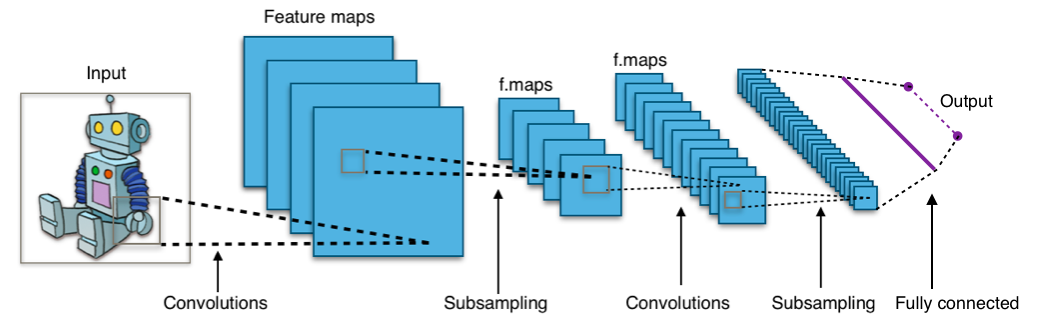
\includegraphics[width=0.95\textwidth]{resources/cnn/typical_cnn}
	\caption{Beispiel CNN Arhcitektur \cite{typical_cnn_img}}
	\label{img:cnn_example_network}
\end{figure}

\section{Verwandte Arbeiten}
TODO \clearpage
% \chapter{Analyse}
Robot Operating System \cite{288}
\newline
Tensorflow \cite{Abadi:2016:TSL:3026877.3026899}

\section{Beispiel Unterkapitel}
TODO

\section{Beispiel Unterkapitel}
TODO \clearpage
\chapter{Konzeption}
TODO

\section{Prior Work TODO}
nur benötigt, wenn die Arbeit auf einer vorherigen aufbaut.

\section{Beispiel Unterkapitel}
TODO

\subsection{Beispiel Unterkapitel zweiter Ebene}
Formelbeispiel
\begin{equation}
	\pi_\theta(s, a) = P [a | s, \theta]
\end{equation}
wobei, $s$ den Zustand repräsentiert, $a$ die Aktion und $\theta$ ... \clearpage
\chapter{Implementierung}
\label{cha:implmentation}
Code Biespiel and Referenze: Code \ref{lst:tf_graph_save}. Nicht geeignet für große Code Biespiele. Verwenden Sie hierfür dne Anhang. Lediglich sehr relevante Kurzzeiler können auf diese Weise dargestellt werden. 
\begin{lstlisting}[caption={Klasse Agent - Tensorflow Graph}, captionpos=b, label={lst:tf_graph_save}]
from keras import backend as k
...
def __init__(...):
	...
	self.graph = k.get_session().graph
	...
\end{lstlisting}

\section{Beispiel Unterkapitel}
TODO

\section{Beispiel Unterkapitel}
TODO \clearpage
\chapter{Experimente}
In diesem Kapitel werden Experimente mit den drei Datensätze durchgeführt. Ebenfalls werden verschiedene Hyperparameter getestet.

\section{Spiel-Datensatz Experimente}
Als erstes wird die Methode auf dem Spiel-Datensatz angewendet. Hiermit soll geprüft werden ob die Methode die erwartete
Ergebnisse liefert. Das U-Net wird für 100 Epochen mit Adam, eine Lernrate von 0.001 und die Cross Entropy Loss Function trainiert. Dieser
Einstellung erwies die besten Ergebnisse. Außerdem wurde ein Experiment mit 36 und ein mit 324 Bins durchgeführt, was kein Einfluss auf die 
Ergebnisse vorwies. Es kann davon ausgegangen werden, dass bei der niedrige Anzahl an möglichen Farben, ein Unterschied bei 36 und 324 Bins
nicht zu erkennen ist. Die unteren Ergebnissen wurden mit 324 Bins erstellt.

\begin{figure}[H]
  \vspace{1cm}
  \begin{subfigure}
    \centering
    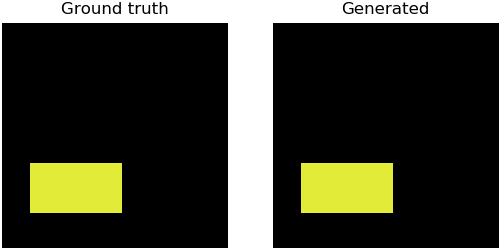
\includegraphics[width=.32\textwidth]{resources/experiments/30.png}
  \end{subfigure}
  \begin{subfigure}
    \centering
    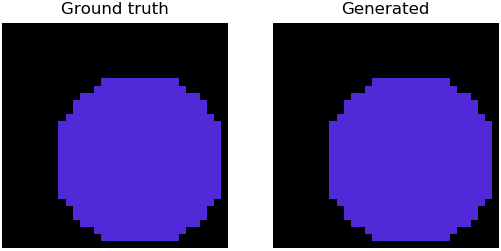
\includegraphics[width=.32\textwidth]{resources/experiments/31.png}
  \end{subfigure}
  \begin{subfigure}
    \centering
    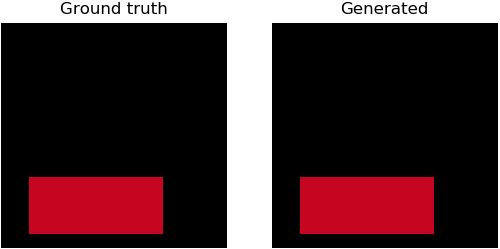
\includegraphics[width=.32\textwidth]{resources/experiments/42.png}
  \end{subfigure}
  \caption{Beispiele von sehr gute Ergebnisse aus dem Spiel-Datensatz}
  \label{image:gute-ergebnisse-toy-dataset}
\end{figure}

Bei den oberen Ergebnisse wurden alle Pixeln richtig klassifiziert, was bei der Größe des Datensatzes oft zu overfitting deutet.
Die unteren Ergebnissen zeigen dass das Model generalisiert und nicht overfited hat.

\begin{figure}[H]
  \vspace{1cm}
  \begin{subfigure}
    \centering
    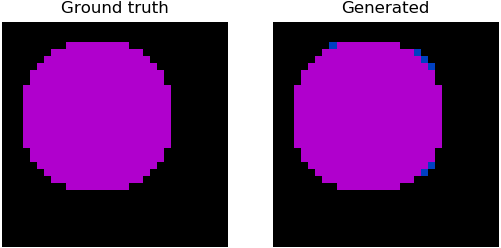
\includegraphics[width=.32\textwidth]{resources/experiments/581.png}
  \end{subfigure}
  \begin{subfigure}
    \centering
    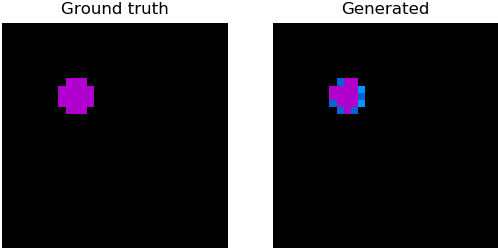
\includegraphics[width=.32\textwidth]{resources/experiments/712.png}
  \end{subfigure}
  \begin{subfigure}
    \centering
    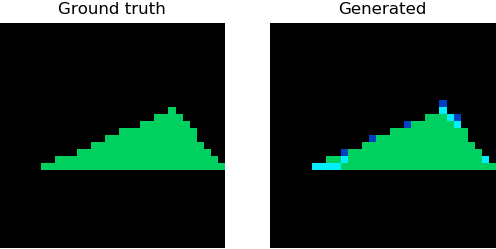
\includegraphics[width=.32\textwidth]{resources/experiments/761.png}
  \end{subfigure}
  \caption{Beispiele von generalisierte Ergebnisse}
  \label{image:nicht-gute-ergebnisse-toy-dataset}
\end{figure}

Das Model zeigte bei einige Ergebnisse, Schwierigkeiten die Pixeln am Rand der geometrische Formen, richtig zu klassifizieren.
Dies tritt speziell auf die Kreise und Dreiecke wo die Ränder nicht aus glatte Linien bestehen. Des weiteren wurden die Farben mittels
den Durchschnitt für jeden möglichen Bin über alle Farben von jeden Trainingsbild rekonstruiert. Ein Unterschied zwischen der Modus und der 
Durchschnitt könnte nicht erkannt werden, da beide Werte gleich waren.
\\
Die Ergebnisse bestätigen dass das Binning und die Methode funktionieren. Anschließend wurden Experimente auf komplexere Bilder
von dem Subset von CIFAR-100 durchgeführt.

\section{CIFAR-100 Subset Experimente}
Das Model wurde auf 12 Klassen von CIFAR-100 über 100 Epochen mit Adam, eine Lernrate von 0.001 und die Cross Entropy Loss Function
trainiert. Diese Einstellungen ergab sich als die beste Kombination von Hyperparameter, jedoch wurde das Training bei unter 50 Epochen unterbrochen
um overfitting zu verhindern.
% Um diesen Anstieg zu vermeiden, wurde ein Mechanismus eingeführt um die Lernrate bei einem bestimmten
% Faktor zu reduzieren wenn der Validation Loss nicht mehr sinkt oder sogar steigt. Dieser Mechanismus bietet PyTorch und wurde mit der 
% Klasse \textit{ReduceLROnPlateau} implementiert.

\begin{figure}[H]
  \centering
  \vspace{1cm}
  \begin{subfigure}
    \centering
    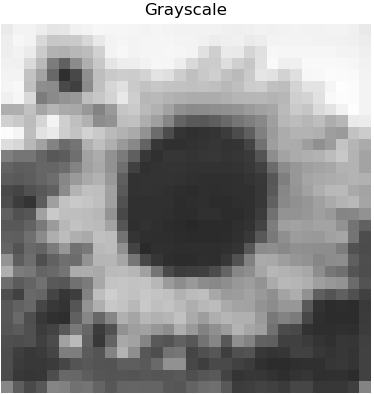
\includegraphics[width=.24\textwidth]{resources/experiments/cifar/200_grayscale.png}
  \end{subfigure}
  \begin{subfigure}
    \centering
    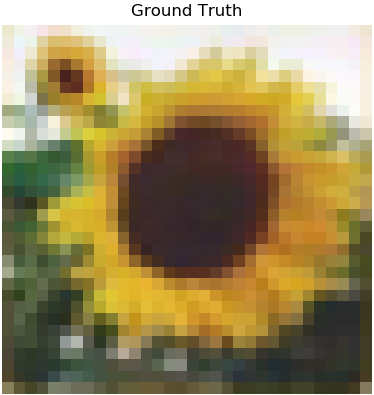
\includegraphics[width=.24\textwidth]{resources/experiments/cifar/200_original.png}
  \end{subfigure}
  \begin{subfigure}
    \centering
    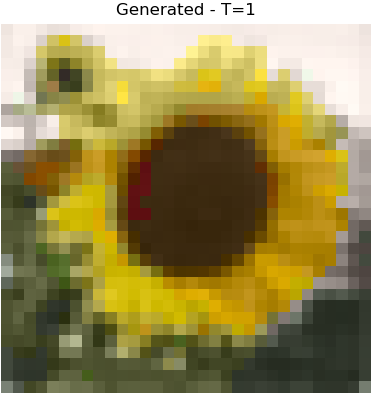
\includegraphics[width=.24\textwidth]{resources/experiments/cifar/200_t1.png}
  \end{subfigure}

  \begin{subfigure}
    \centering
    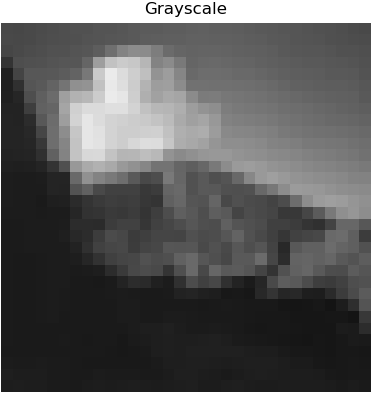
\includegraphics[width=.24\textwidth]{resources/experiments/cifar/600_grayscale.png}
  \end{subfigure}
  \begin{subfigure}
    \centering
    
\includegraphics[width=.24\textwidth]{resources/experiments/cifar/600_original.png}
  \end{subfigure}
  \begin{subfigure}
    \centering
    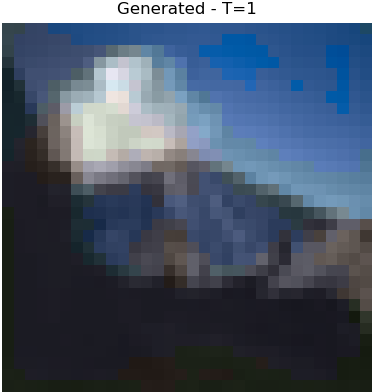
\includegraphics[width=.24\textwidth]{resources/experiments/cifar/600_t1.png}
  \end{subfigure}
  \caption{Beispiele von gute Ergebnisse aus dem Subset von CIFAR-100 mit 324 Bins. Die erste Spalte beinhaltet das Graustufenbild, die zweite Spalte
  beinhaltet das Originale Bild und die letzte Spalte stellt das generierte Bild dar. Das generierte Bild wurde mit eine Temperatur von 1
  erzeugt, was bedeutet dass die rekonstruierte Farben den Durchschnitt aus jedem Bin repräsentieren.}
  \label{image:gute-ergebnisse-cifar}
\end{figure}

Die Experimente mit diesem Datensatz haben gezeigt dass die Anzahl der Bins bei der Auswahl an möglichen Farben die Ergebnisse beeinträchtigen.
Eine Erhöhung an Trainingszeit zwischen 36 und 324 Bins war nicht zu erkennen.

% TODO: Change image
\begin{figure}[H]
  \centering
  \vspace{1cm}
  \begin{subfigure}
    \centering
    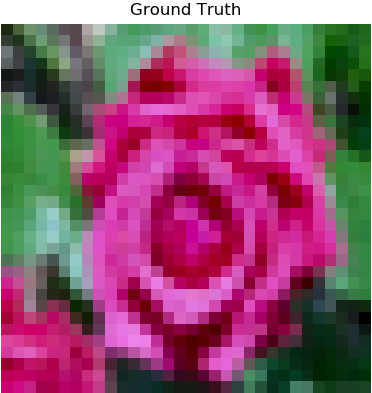
\includegraphics[width=.24\textwidth]{resources/experiments/cifar/12_original.png}
  \end{subfigure}
  \begin{subfigure}
    \centering
    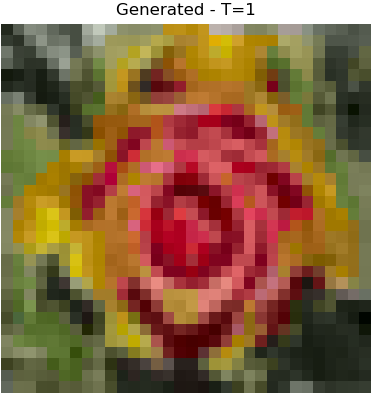
\includegraphics[width=.24\textwidth]{resources/experiments/cifar/12_t1.png}
  \end{subfigure}
  \begin{subfigure}
    \centering
    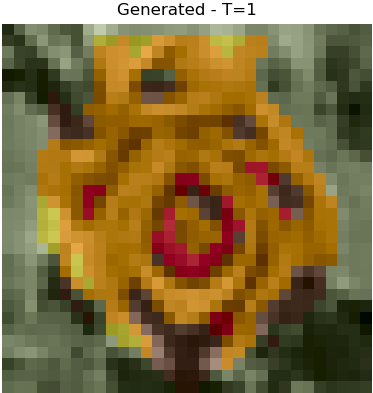
\includegraphics[width=.24\textwidth]{resources/experiments/cifar/12_t1_36.png}
  \end{subfigure}

  \caption{Einfluss von Anzahl der Bins auf die Ergebnisse. Das zweite Bild wurde mit 324 Bins generiert, das dritte nur mit 36.}
  \label{image:gute-ergebnisse-cifar}
\end{figure}

Um das Overfitting zu verhindern wurden Zahlreiche Experimente mit verschiedene Optimierer, Aktivierungsfunktionen und Lernraten durchgeführt.
Eine Ersetzung von ReLU durch Tanh zeigte ein stabilerer Trainingsverhalten aber eine Verschlechterung der Validation Loss. Leaky ReLU zeigte 
ein ähnliches Verhalten wie ReLU aber keine Verbesserung. Die Verwendung von RMSprop anstatt Adam zeigte eine langsamere Konvergenz Richtung Minimum.
Abschließend wurden die Anzahl der Filter in den Convolutional Layers halbiert was eine positive Wirkung auf das Training zeigte.   

\subsection{Experimente mit MSE Loss und ohne Binning}
Um die Performance von Klassifikation gegenüber Regression zu messen, wurde ein Model mit der MSE Loss Function trainiert. Dieses Model
wurde ebenfalls mit den gleichen Parameter wie das Klassifikationsmodell trainiert und hat beeindruckende Ergebnisse erreicht. Einige Ergebnisse
zeigten Blasse stellen im Vergleich zu das Klassifikationsmodell, der leuchtende Farben an den gleichen Stellen gezeigt hat.

\begin{figure}[H]
  \centering
  \vspace{1cm}
  \begin{subfigure}
    \centering
    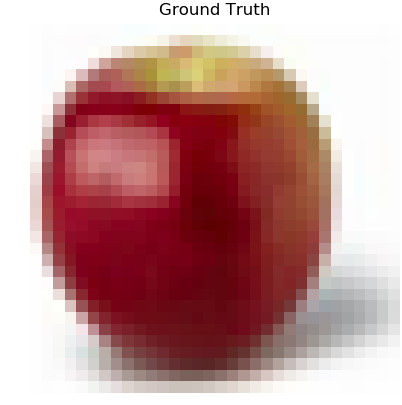
\includegraphics[width=.28\textwidth]{resources/experiments/cifar/311_original.png}
  \end{subfigure}
  \begin{subfigure}
    \centering
    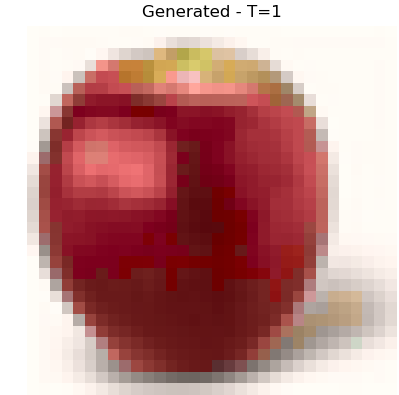
\includegraphics[width=.28\textwidth]{resources/experiments/cifar/311_t1.png}
  \end{subfigure}
  \begin{subfigure}
    \centering
    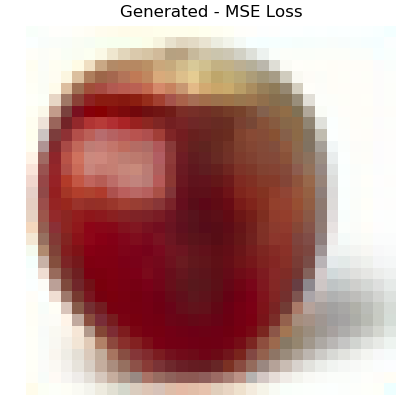
\includegraphics[width=.28\textwidth]{resources/experiments/cifar/311_regression.png}
  \end{subfigure}

  \caption{Vergleich von Klassifikation mit Binning gegenüber Regression. Das zweite Bild wurde mit 324 Bins und der Cross Entropy Loss generiert.
  Das dritte Bild wurde ohne Binning und mit einem MSE Loss generiert.}
  \label{image:gute-ergebnisse-cifar}
\end{figure}

\section{Landscape Datensatz Experimente}
Dieser Datensatz wurde anhand der Hyperparameter Optimierung von den CIFAR-100 Subset trainiert. Es wurde das größere Model für $128 \times 128$
Input Bilder angewendet. Das Model wurde ebenfalls für 36 und 324 Bins, mit dem Adam Optimizer, eine Lernrate von 0.001 und die Cross Entropy 
Loss Function für 60 Epochen trainiert. Das Model mit den besten Validation Loss wurde gespeichert um die Ergebnisse zu evaluieren. Außerdem
wurden den Einfluss der Temperaturwert und der Anzahl der Bins auf die Ergebnisse gemessen.

\begin{figure}[H]
  \centering
  \vspace{1cm}
  \begin{subfigure}
    \centering
    \includegraphics[width=.235\textwidth]{resources/experiments/landscape/043/043_original.png}
  \end{subfigure}
  \begin{subfigure}
    \centering
    \includegraphics[width=.235\textwidth]{resources/experiments/landscape/043/043_t0.png}
  \end{subfigure}
  \begin{subfigure}
    \centering
    \includegraphics[width=.235\textwidth]{resources/experiments/landscape/043/043_t08.png}
  \end{subfigure}
  \begin{subfigure}
    \centering
    \includegraphics[width=.235\textwidth]{resources/experiments/landscape/043/043_t1.png}
  \end{subfigure}

  \begin{subfigure}
    \centering
    \includegraphics[width=.235\textwidth]{resources/experiments/landscape/253/253_original.png}
  \end{subfigure}
  \begin{subfigure}
    \centering
    \includegraphics[width=.235\textwidth]{resources/experiments/landscape/253/253_t0.png}
  \end{subfigure}
  \begin{subfigure}
    \centering
    \includegraphics[width=.235\textwidth]{resources/experiments/landscape/253/253_t08.png}
  \end{subfigure}
  \begin{subfigure}
    \centering
    \includegraphics[width=.235\textwidth]{resources/experiments/landscape/253/253_t1.png}
  \end{subfigure}

  \caption{Ergebnisse mit 324 Bins. Die erste Spalte zeigt das Originale Bild, die zweite zeigt das generierte Bild mit einer Temperatur von 0 
  (Modus der jeweiligen Bin), die dritte Spalte zeigt das generierte Bild mit einer Temperatur von 0.8 (Modus der jeweiligen Bin minus 
  80\% der Distanz zwischen Modus und Durchschnitt) und die vierte Spalte zeigt das generierte Bild mit einer Temperatur von 1 
  (Durchschnitt der jeweiligen Bin)}
  \label{image:gute-ergebnisse-cifar}
\end{figure}

Das Model tendierte ebenfalls bei diesem Datensatz zum Overfitting. Um das zu verhindern wurden die gleiche Techniken wie bei CIFAR-100
angewendet, was keine bessere Ergebnisse geliefert hat. Eine Halbierung der Anzahl der Filter bei den Convolutional Layers erwiesen eine Verschlechterung
des Validation Loss und half nicht bei Overfitting. Eine Änderung der Optimierer zu RMSprop und die Ersetzung von ReLU für Tanh zeigten
einen stabileren Training aber keine Verbesserung der Validation Loss. Das Endgültige Model wurde trainiert bis der Validation Loss wieder stieg.
 \clearpage
\chapter{Evaluation}
\label{sec:evaluation}
TODO

\section{Beispiel Unterkapitel}
Beispiel einer Tabelle:
\begin{longtable}{|c|c|c|c|}
	\hline
	\multicolumn{1}{|c}{\textbf{Spalte 1}} &
	\multicolumn{1}{|c}{\textbf{Spalte 2}} &
	\multicolumn{1}{|c|}{\textbf{Spalte 3}} \\
	\hline
	\endfirsthead
	
	\multicolumn{3}{c}{Beschreibung}\\ \hline
	\multicolumn{1}{|c}{\textbf{Spalte 1}} &
	\multicolumn{1}{|c}{\textbf{Spalte 2}} &
	\multicolumn{1}{|c|}{\textbf{Spalte 3}} \\
	\hline
	\endhead
	
	\multicolumn{2}{c}{Fortsetzugn auf der nächsten Seite}
	\endfoot
	
	\caption{Beschreibung}
	\label{tab:example}
	\endlastfoot
	
	TODO & TODO & TODO \\ \hline
	TODO & TODO & TODO  \\ \hline
\end{longtable}

\section{Beispiel Unterkapitel}
TODO \clearpage
\chapter{Fazit}
TODO

\section{Zusammenfassung}
TODO

\section{Kritischer Rückblick}
TODO (Reflexion und Bewertung der Zielsetzung gegenüber erreichtem Ergebnis)

\section{Ausblick}
TODO \clearpage

\pagenumbering{Roman}
% List of Figures
\listoffigures \clearpage
% List of Tables
\listoftables \clearpage
% Source Code Content
\lstlistoflistings \clearpage

\printindex \clearpage

\printnoidxglossary[title=Glossar] \clearpage

\defbibfilter{scientific}{
	type=article or
	type=inbook or
	type=book or
	type=unpublished or
	type=inproceedings or
	type=incollection or
	type=manual or
	type=misc or
	type=phdthesis
}

\printbibliography[heading=bibintoc, filter=scientific, title={Literaturverzeichnis}]\clearpage
\printbibliography[heading=bibintoc, keyword={online}, title={Onlinereferenzen}]\clearpage
\printbibliography[heading=bibintoc, keyword={image}, title={Bildreferenzen}]\clearpage

% Appendix
\appendix
\chapter{}
\addcontentsline{toc}{chapter}{Anhang A}
\section{Beispiel}
\label{code:appendix_example}
TODO

% Eigenständigkeitserklärung (CHOOSE ONE)
\addchap{Eigenständigkeitserklärung}

Hiermit versichere ich, dass ich die vorliegende Bachelorarbeit selbstständig und nur unter Verwendung der angegebenen Quellen und Hilfsmittel verfasst habe. Die Arbeit wurde bisher in gleicher oder ähnlicher Form keiner anderen Prüfungsbehörde vorgelegt.

\vskip 1cm

Berlin, den XX.XX.2018

\vskip 1.5cm

Vorname Nachname


\end{document}
